\section[Algoritmo Divide y Vencerás]{Algoritmo Divide y Vencerás}
\begin{frame}[plain]
	\frametitle{Resolución}
		\begin{exampleblock}{Estrategia de resolución}
			Nos posicionamos sobre el elemento que ocupa la posición media de la estructura:
			\begin{enumerate}
				\item  Si el elemento a su izquierda es mayor y si elemento a la derecha es menor, entonces, nos quedamos con la primera mitad de la estructura.
				\item Si el elemento a su izquierda es menor y su elemento a la derecha es mayor, entonces, nos quedamos con la segunda mitad de la estructura.
				\item Si el elemento a su izquierda es menor y su elemento a la derecha es menor: ¡Hemos encontrado el elemento que buscábamos!
			\end{enumerate}
		\end{exampleblock}
		
\end{frame}		




\begin{frame}[plain]
	\frametitle{Breve explicación - Paso 0}
		\begin{figure}[htb]
		\begin{center}
		\begin{picture}(160,0)
		\put(-110,-100){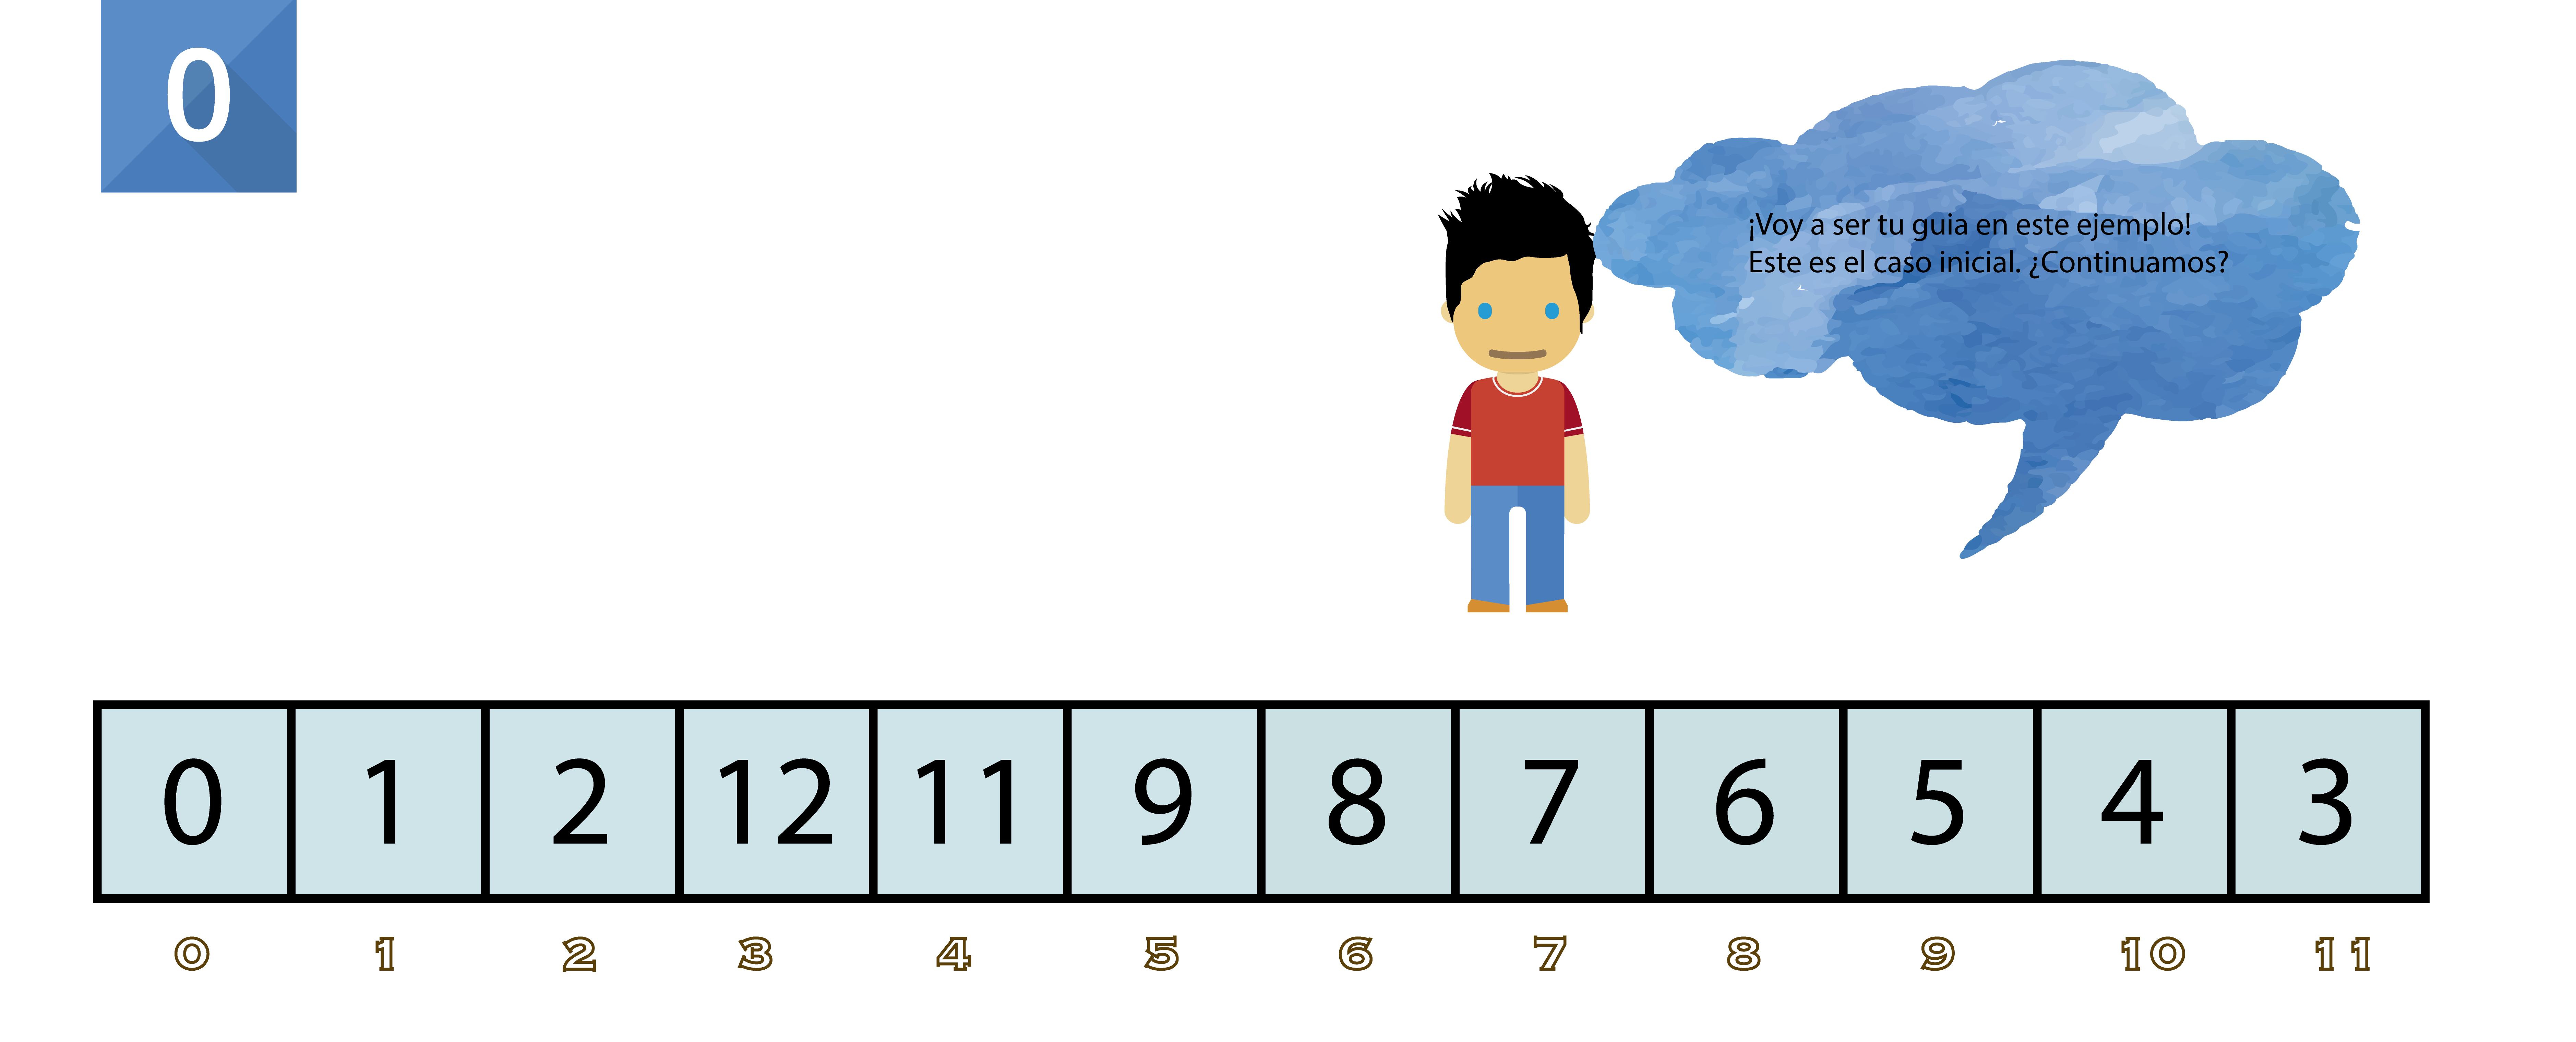
\includegraphics[width=13.5cm,height=6.5cm]{Images/Paso0}}
		\end{picture}
		\end{center}
		\end{figure}
		
\end{frame}	

\begin{frame}[plain]
	\frametitle{Breve explicación - Paso 1}
		\begin{figure}[htb]
		\begin{center}
		\begin{picture}(160,0)
		\put(-110,-100){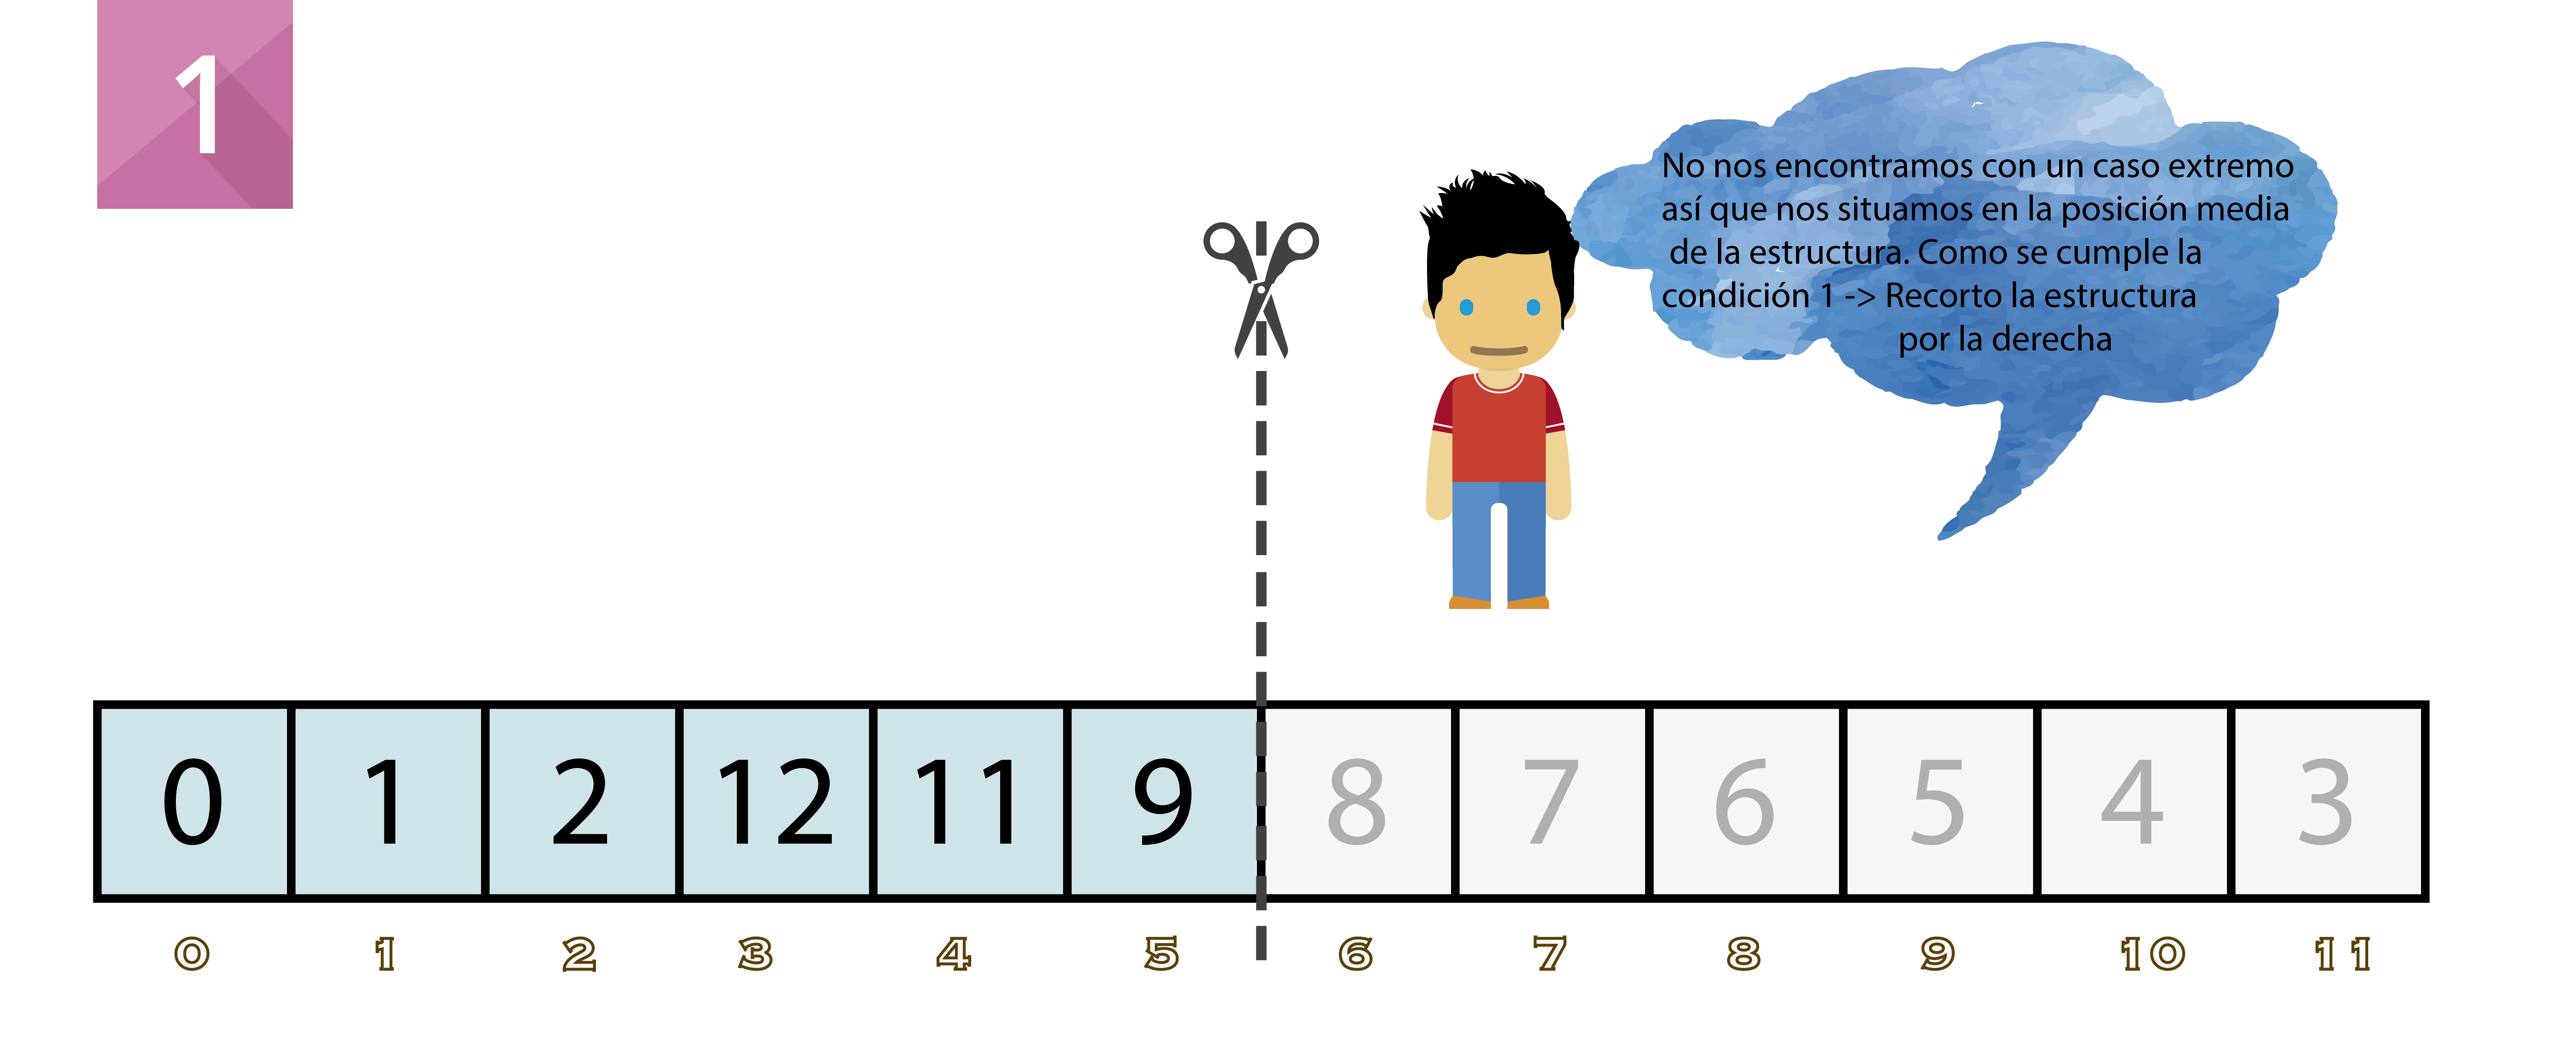
\includegraphics[width=13.5cm,height=6.5cm]{Images/Paso1}}
		\end{picture}
		\end{center}
		\end{figure}
		
\end{frame}	

\begin{frame}[plain]
	\frametitle{Breve explicación - Paso 2}
		\begin{figure}[htb]
		\begin{center}
		\begin{picture}(160,0)
		\put(-110,-100){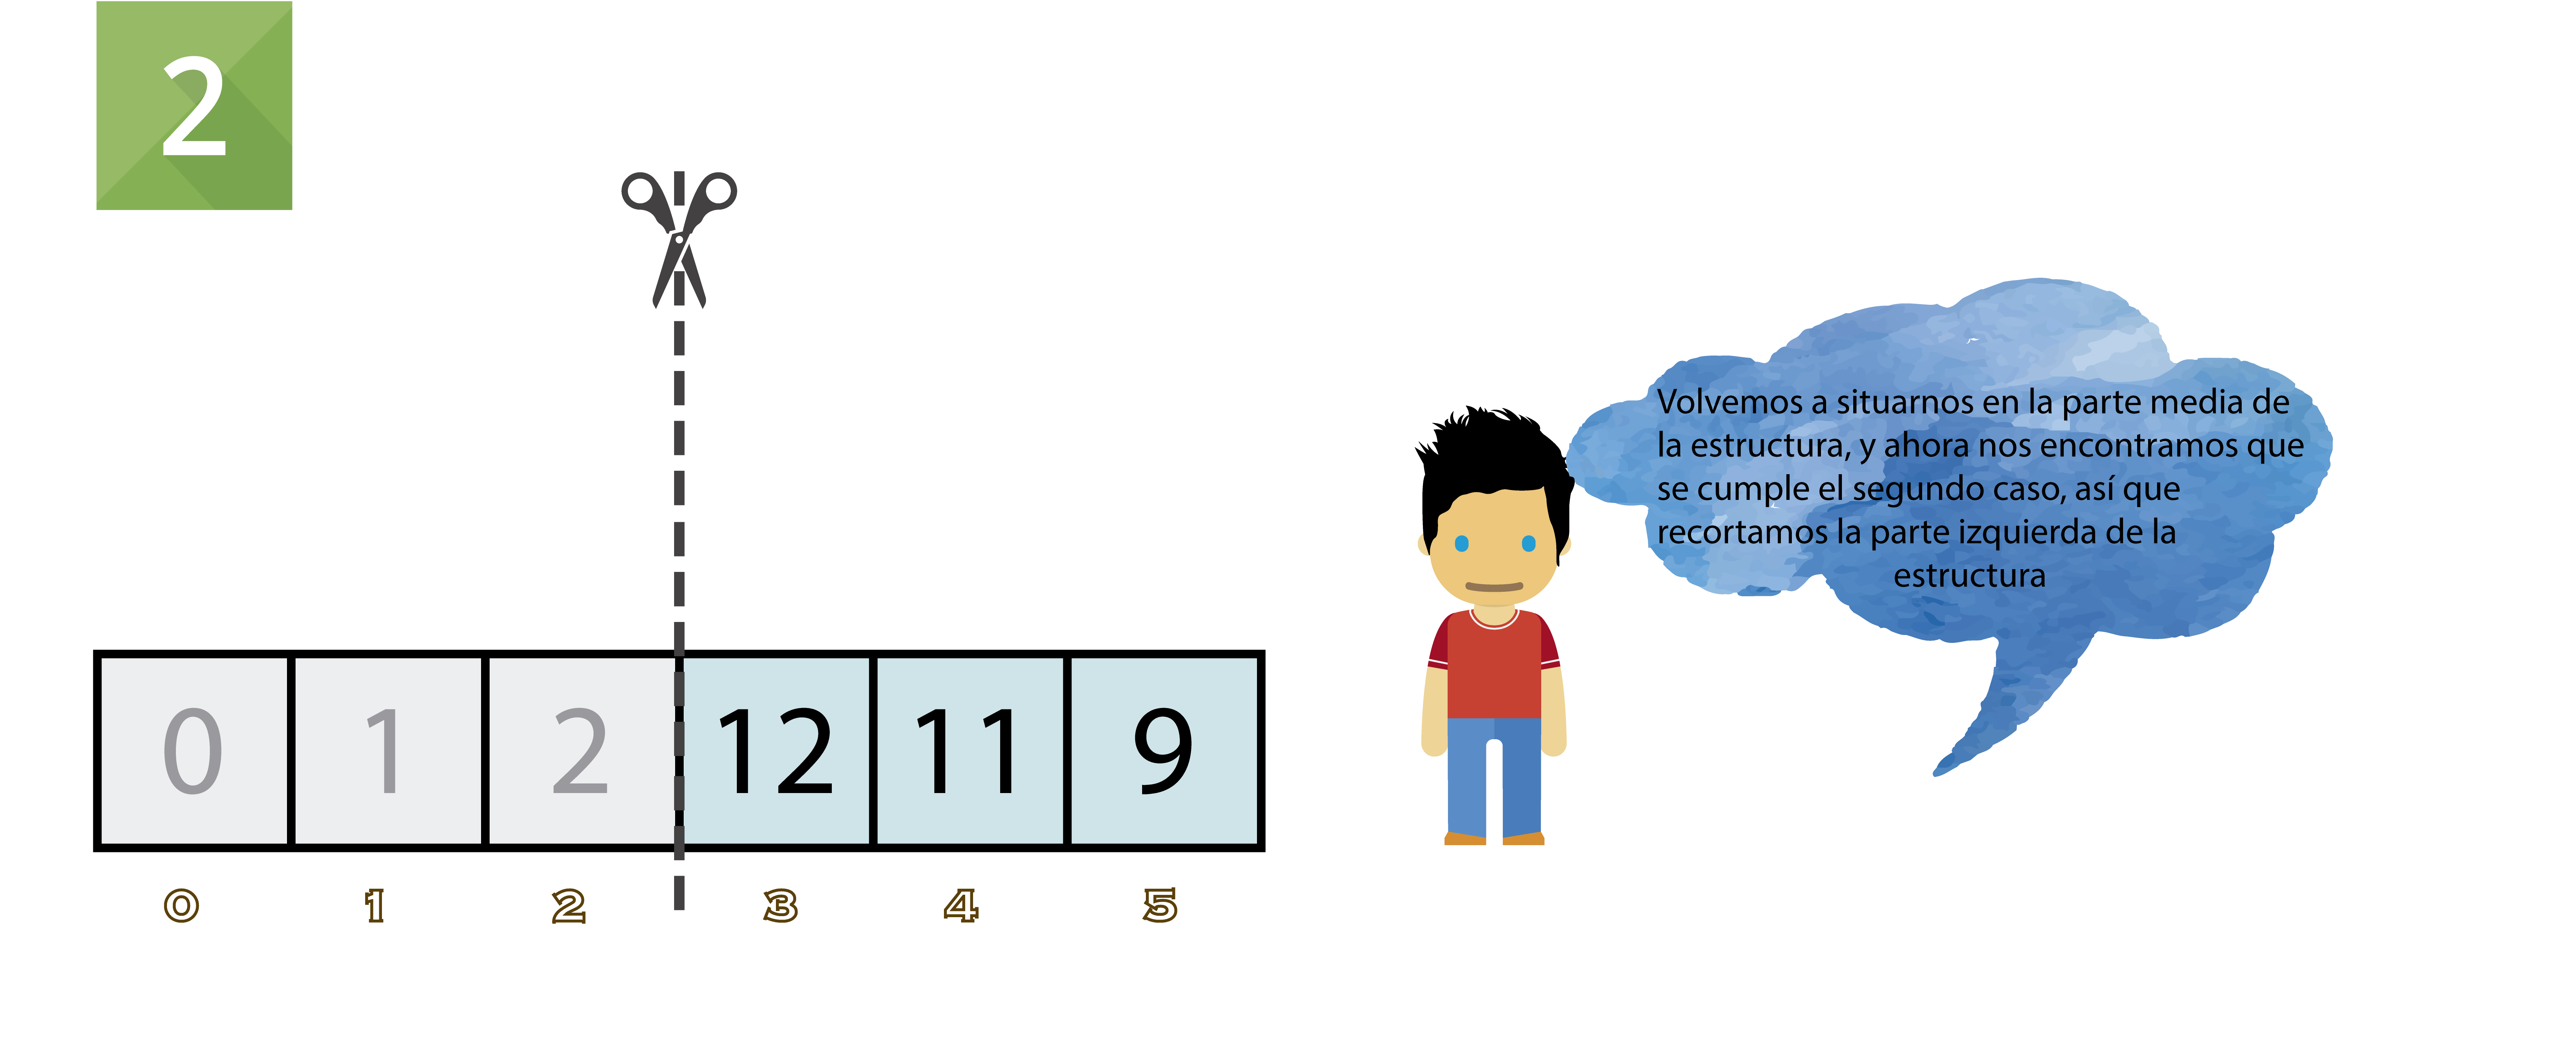
\includegraphics[width=13.5cm,height=6.5cm]{Images/Paso2}}
		\end{picture}
		\end{center}
		\end{figure}
		
\end{frame}	

\begin{frame}[plain]
	\frametitle{Breve explicación - Paso 3}
		\begin{figure}[htb]
		\begin{center}
		\begin{picture}(160,0)
		\put(-110,-100){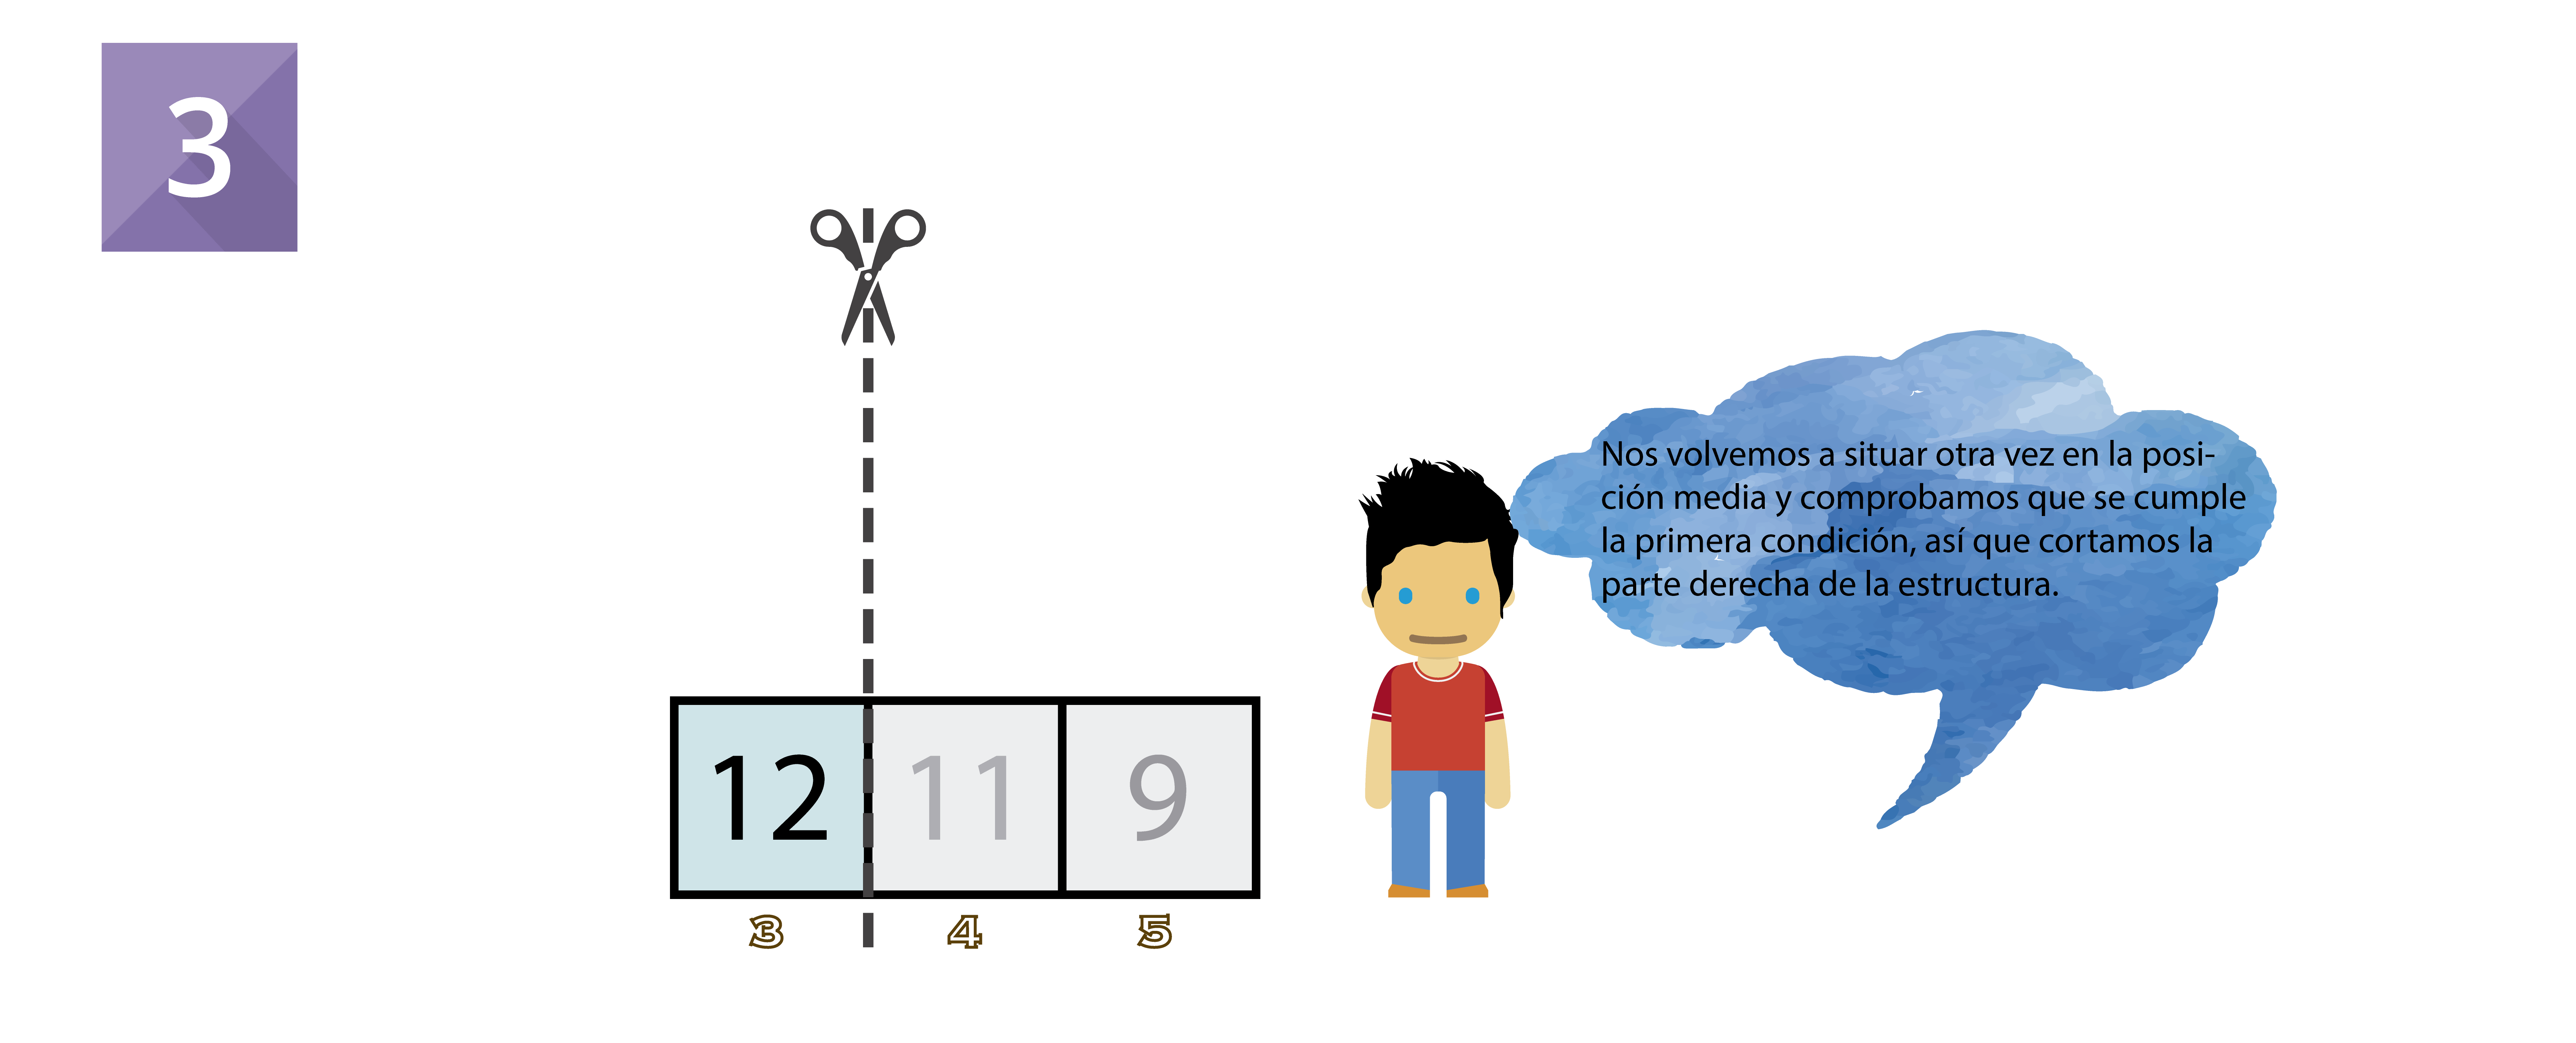
\includegraphics[width=13.5cm,height=6.5cm]{Images/Paso3}}
		\end{picture}
		\end{center}
		\end{figure}
		
\end{frame}	

\begin{frame}[plain]
	\frametitle{Breve explicación - Paso 4}
		\begin{figure}[htb]
		\begin{center}
		\begin{picture}(160,0)
		\put(-110,-100){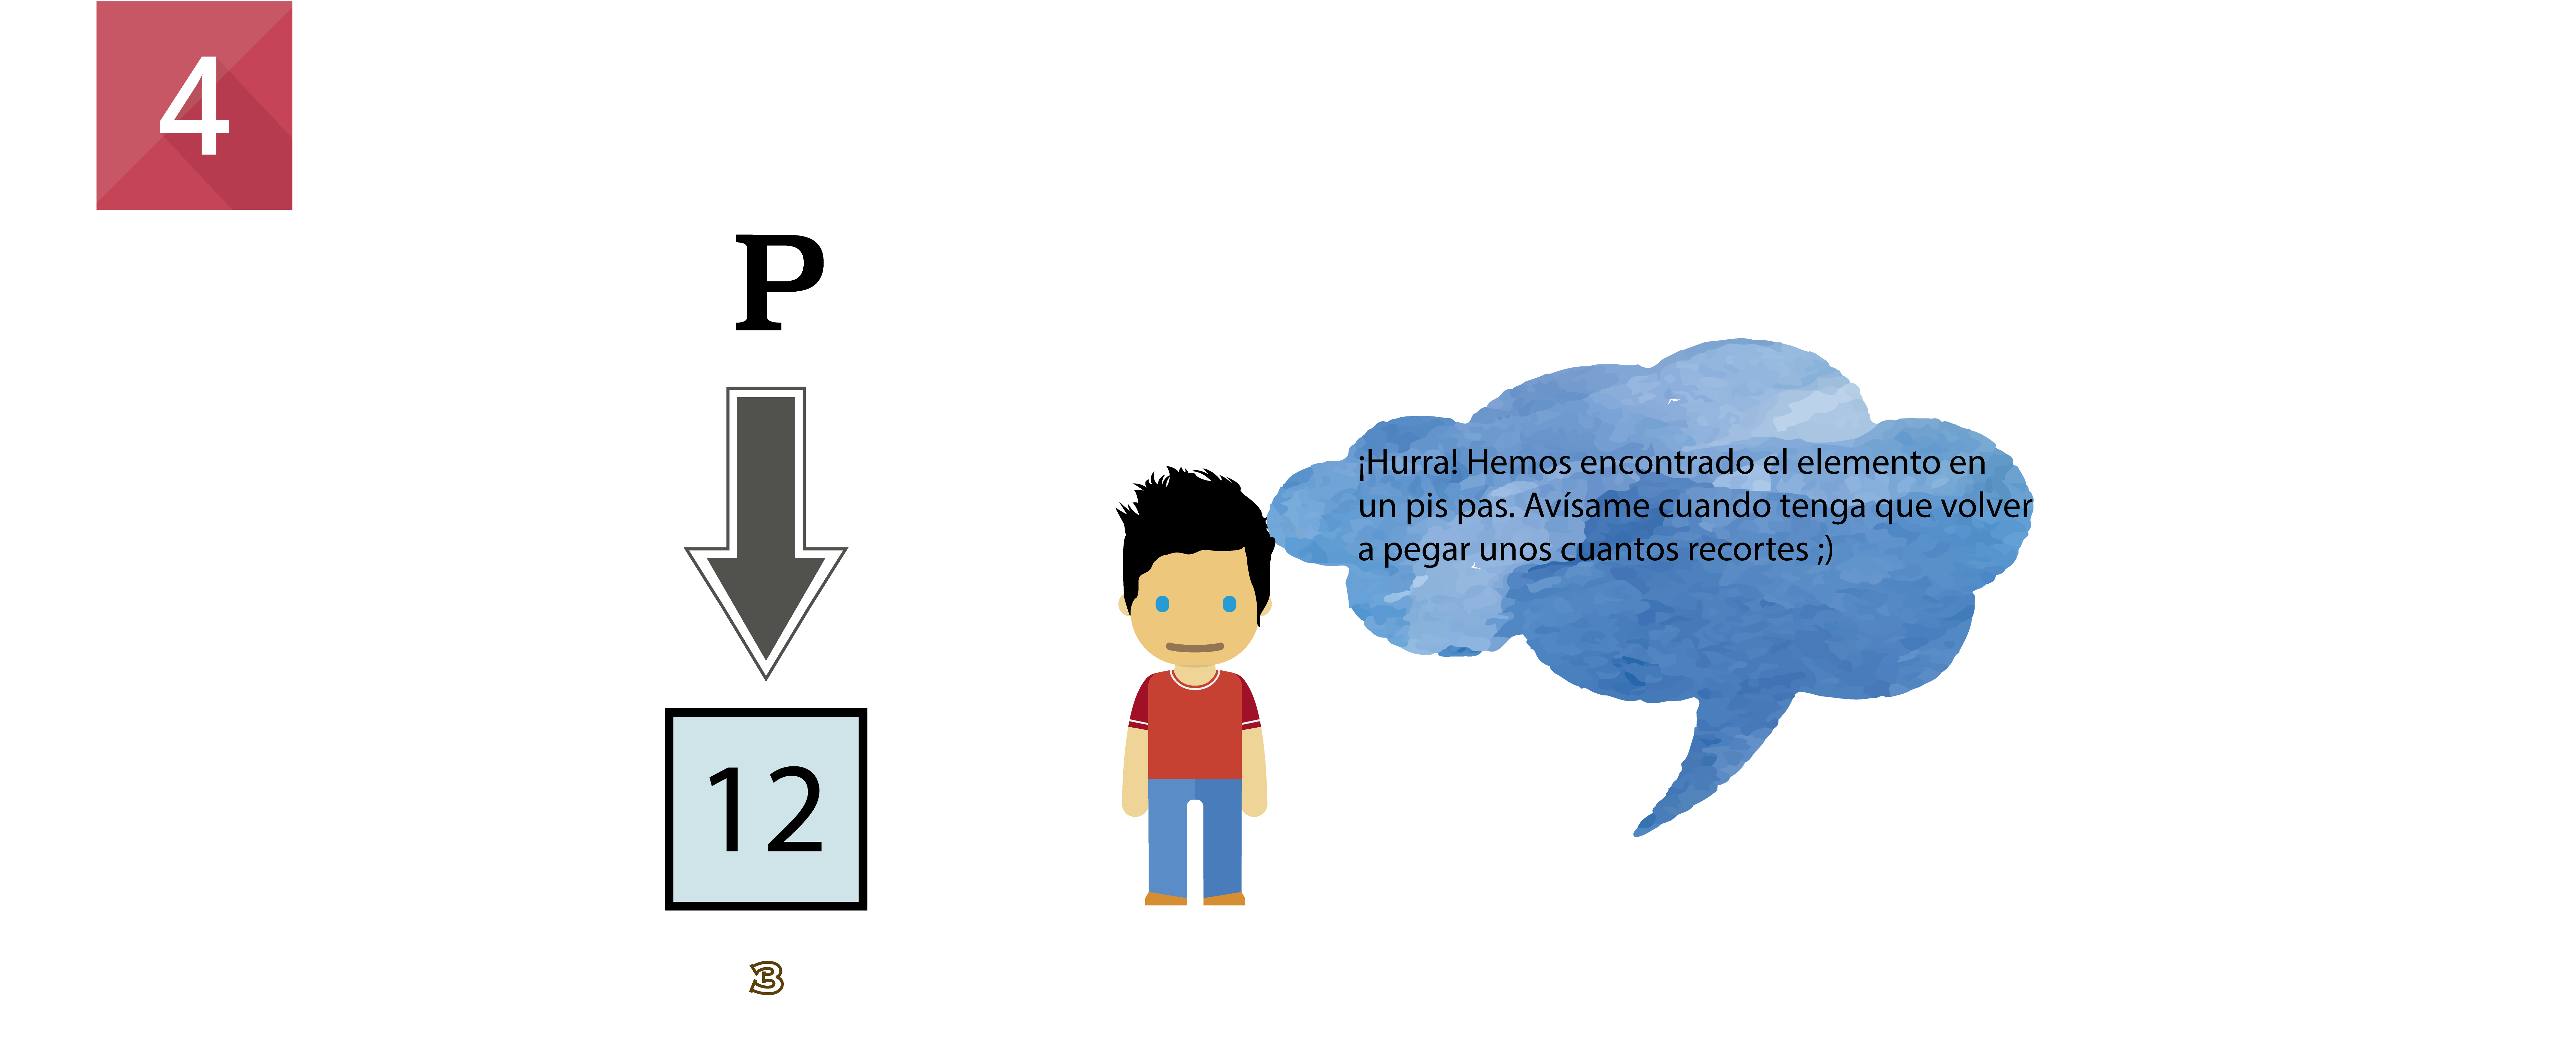
\includegraphics[width=13.5cm,height=6.5cm]{Images/Paso4}}
		\end{picture}
		\end{center}
		\end{figure}
		
\end{frame}	









\begin{frame}[fragile]
	\frametitle{Algoritmo Bruto - Implementación}
	\lstset{language=C++,
                basicstyle=\ttfamily,
                tabsize=3, 
				showstringspaces=false,
				extendedchars=true,
                keywordstyle=\color{blue}\ttfamily,
                stringstyle=\color{red}\ttfamily,
                commentstyle=\color{yellow}\ttfamily,
                basicstyle=\small,
                morecomment=[l][\color{magenta}]{\#}
     }
			\vspace*{-0.1in}
\begin{lstlisting}
int unimodalDyV(vector<int> &v, int inicio, int final){
    int posicionMedia = (inicio + final) / 2;
    bool found = false;
    if(posicionMedia > inicio){
        if(v[posicionMedia-1] > v[posicionMedia] 
        && v[posicionMedia] > v[posicionMedia+1])
             return unimodalDyV(v, inicio, posicionMedia);
        else if(v[posicionMedia-1] < v[posicionMedia] 
        		&& v[posicionMedia] < v[posicionMedia+1])
            return unimodalDyV(v, posicionMedia, final);
        else if(v[posicionMedia] > v[posicionMedia-1] 
        		&& v[posicionMedia+1]<v[posicionMedia])
            return posicionMedia;
    }else{
        if(v[inicio] <= v[final])
            return final;
        else
            return inicio;
    }
}

\end{lstlisting}		
\end{frame}	


\begin{frame}[plain]
	\frametitle{Análisis Híbrido}
		\begin{figure}[htb]
		\begin{center}
		\begin{picture}(160,0)
		\put(-50,-110){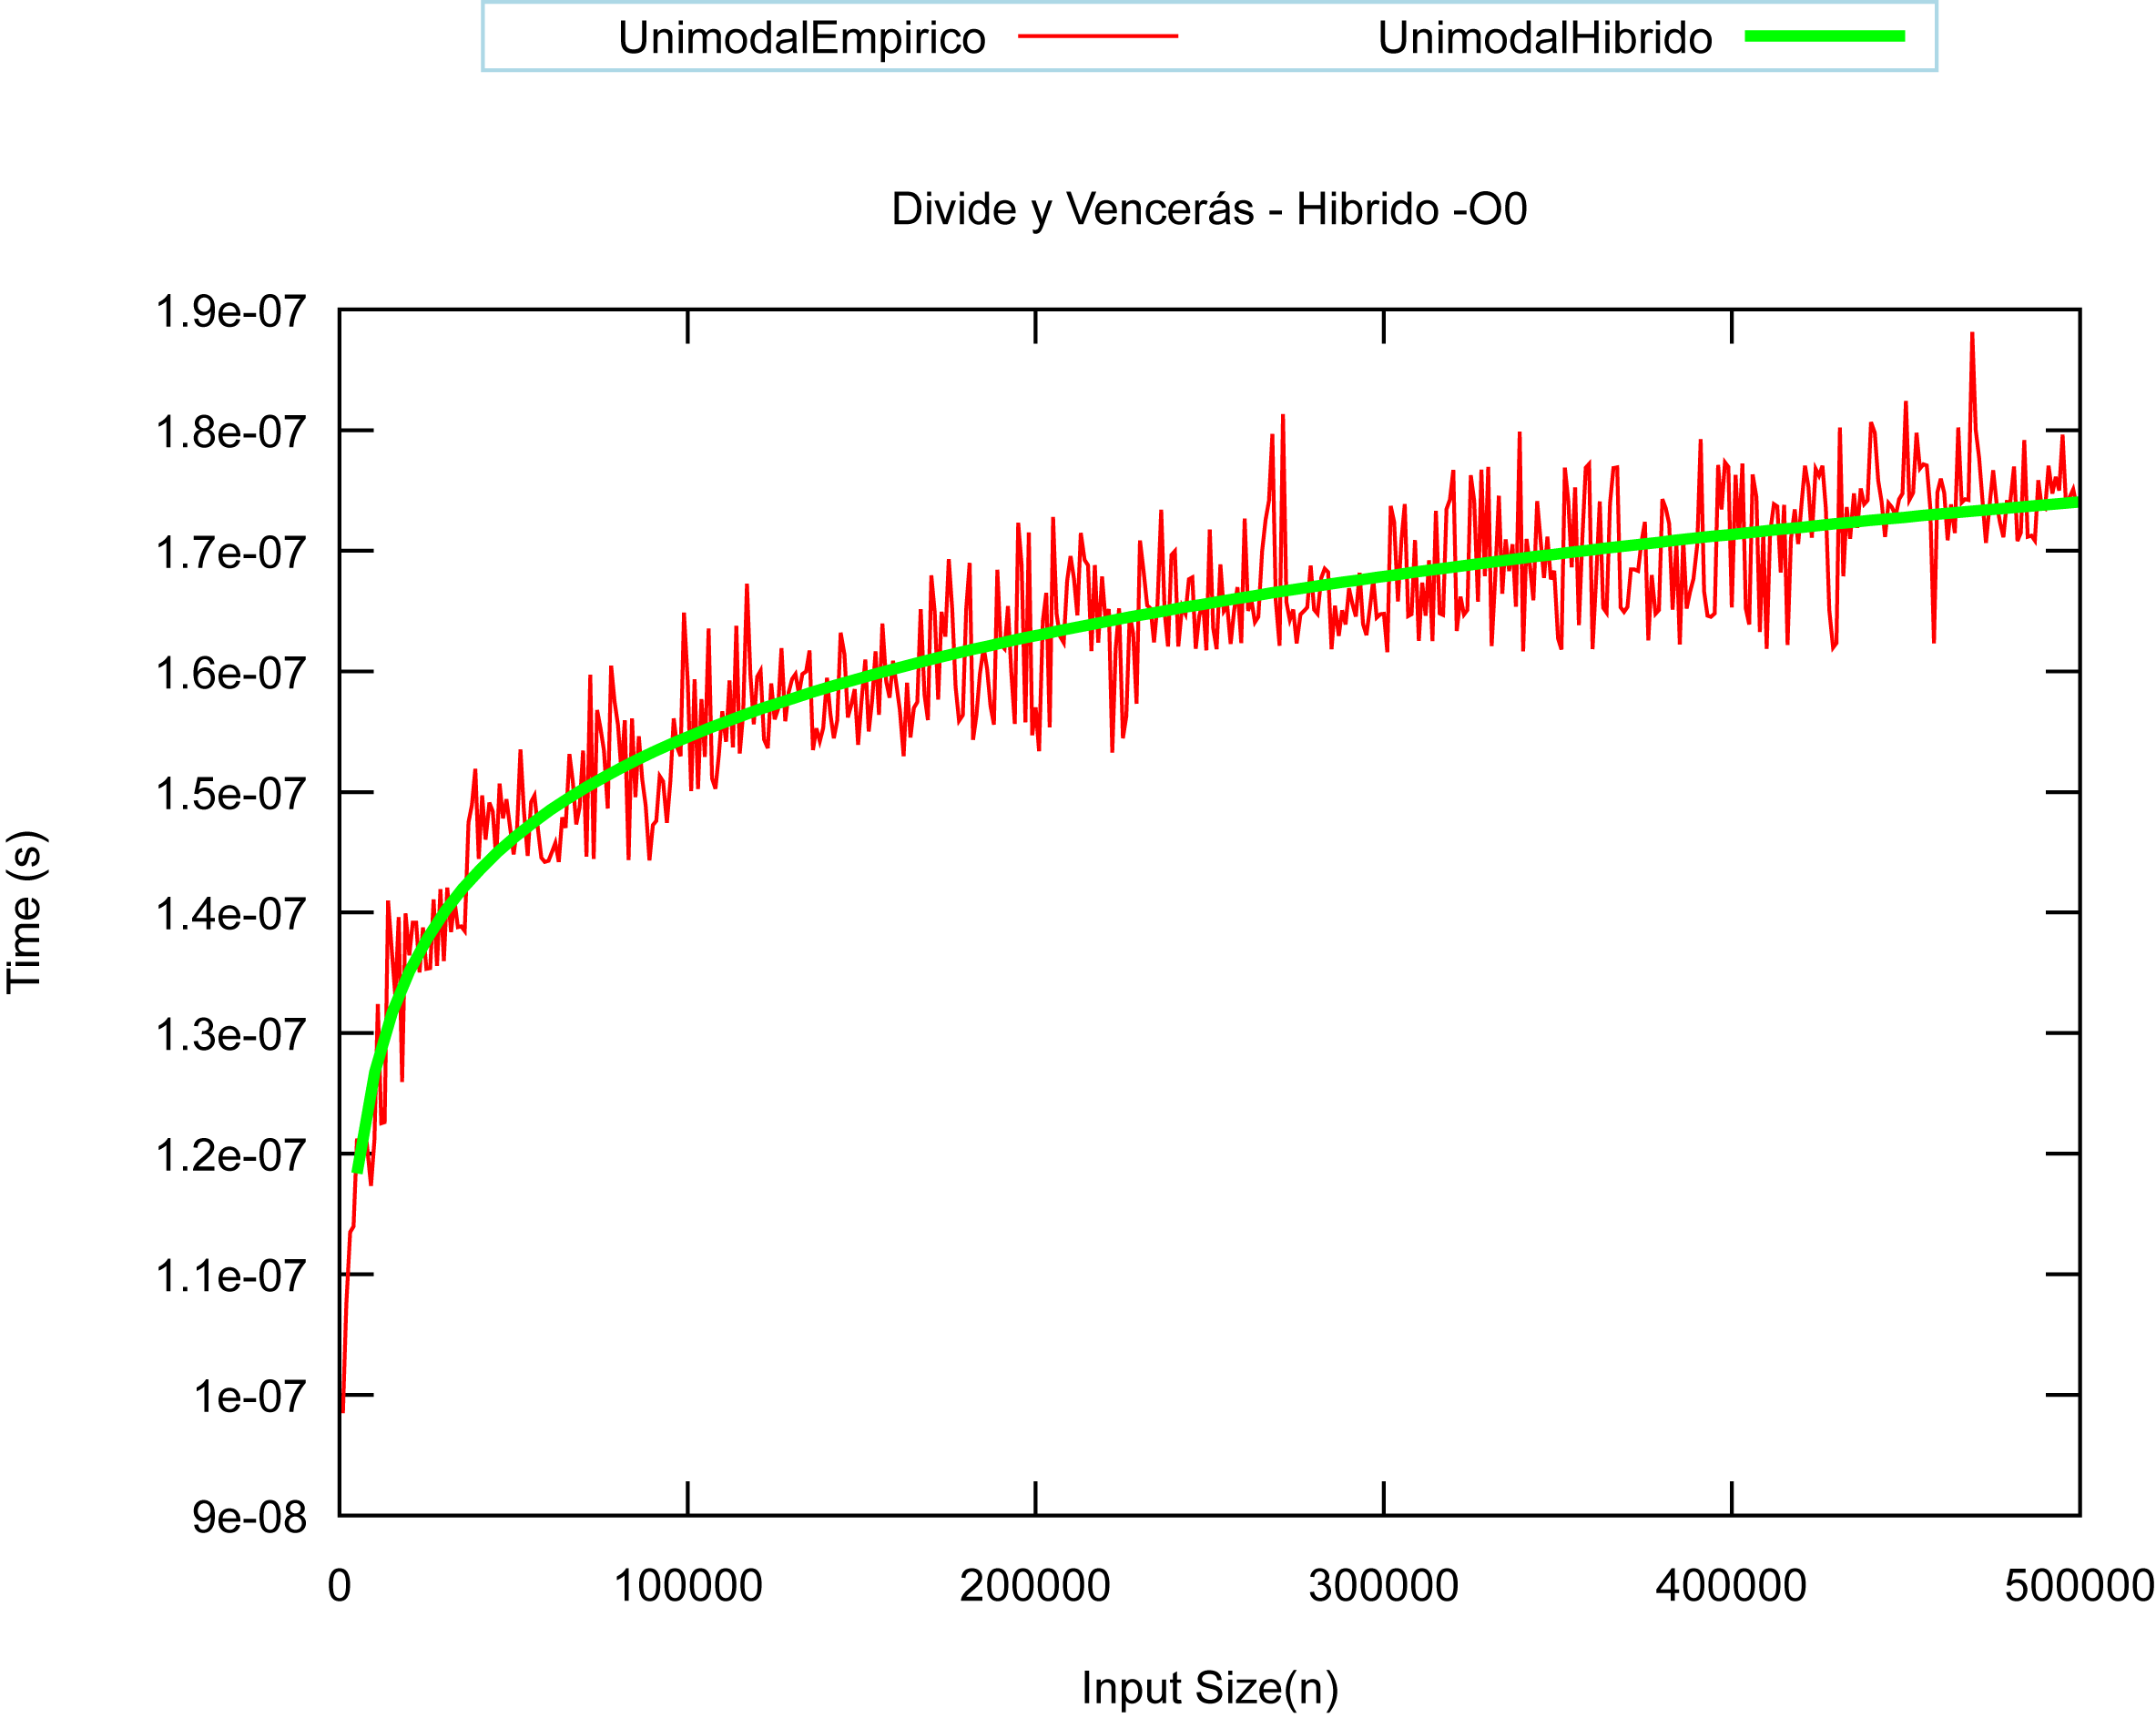
\includegraphics[width=8.6cm,height=7.1cm]{Images/dyv-hibridoO0}}
		\end{picture}
		\end{center}
		\end{figure}
		
\end{frame}	


	
\begin{frame}[plain]
	\frametitle{Constantes ocultas}
	
		\begin{defn}
			
			Sabemos que la función que describe la eficiencia de este algoritmo tiene la siguiente forma:
		\begin{equation}
			T(n)= a\cdot log(n) + b
		\end{equation}
		
		Al realizar el ajuste de los datos con la herramienta \textit{gnuplot} obtenemos el valor de las constantes ocultas, quedando por tanto:
		
		\begin{equation}
			T(n) = 1.21165\cdot 10^{-08} \cdot log(n) + 1.50656\cdot 10^{-08}
		\end{equation}
	
		\vspace*{0.05in}
		
	\end{defn}
		
\end{frame}




\begin{frame}[plain]
	\frametitle{Optimización 1}
		\begin{figure}[htb]
		\begin{center}
		\begin{picture}(160,0)
		\put(-50,-110){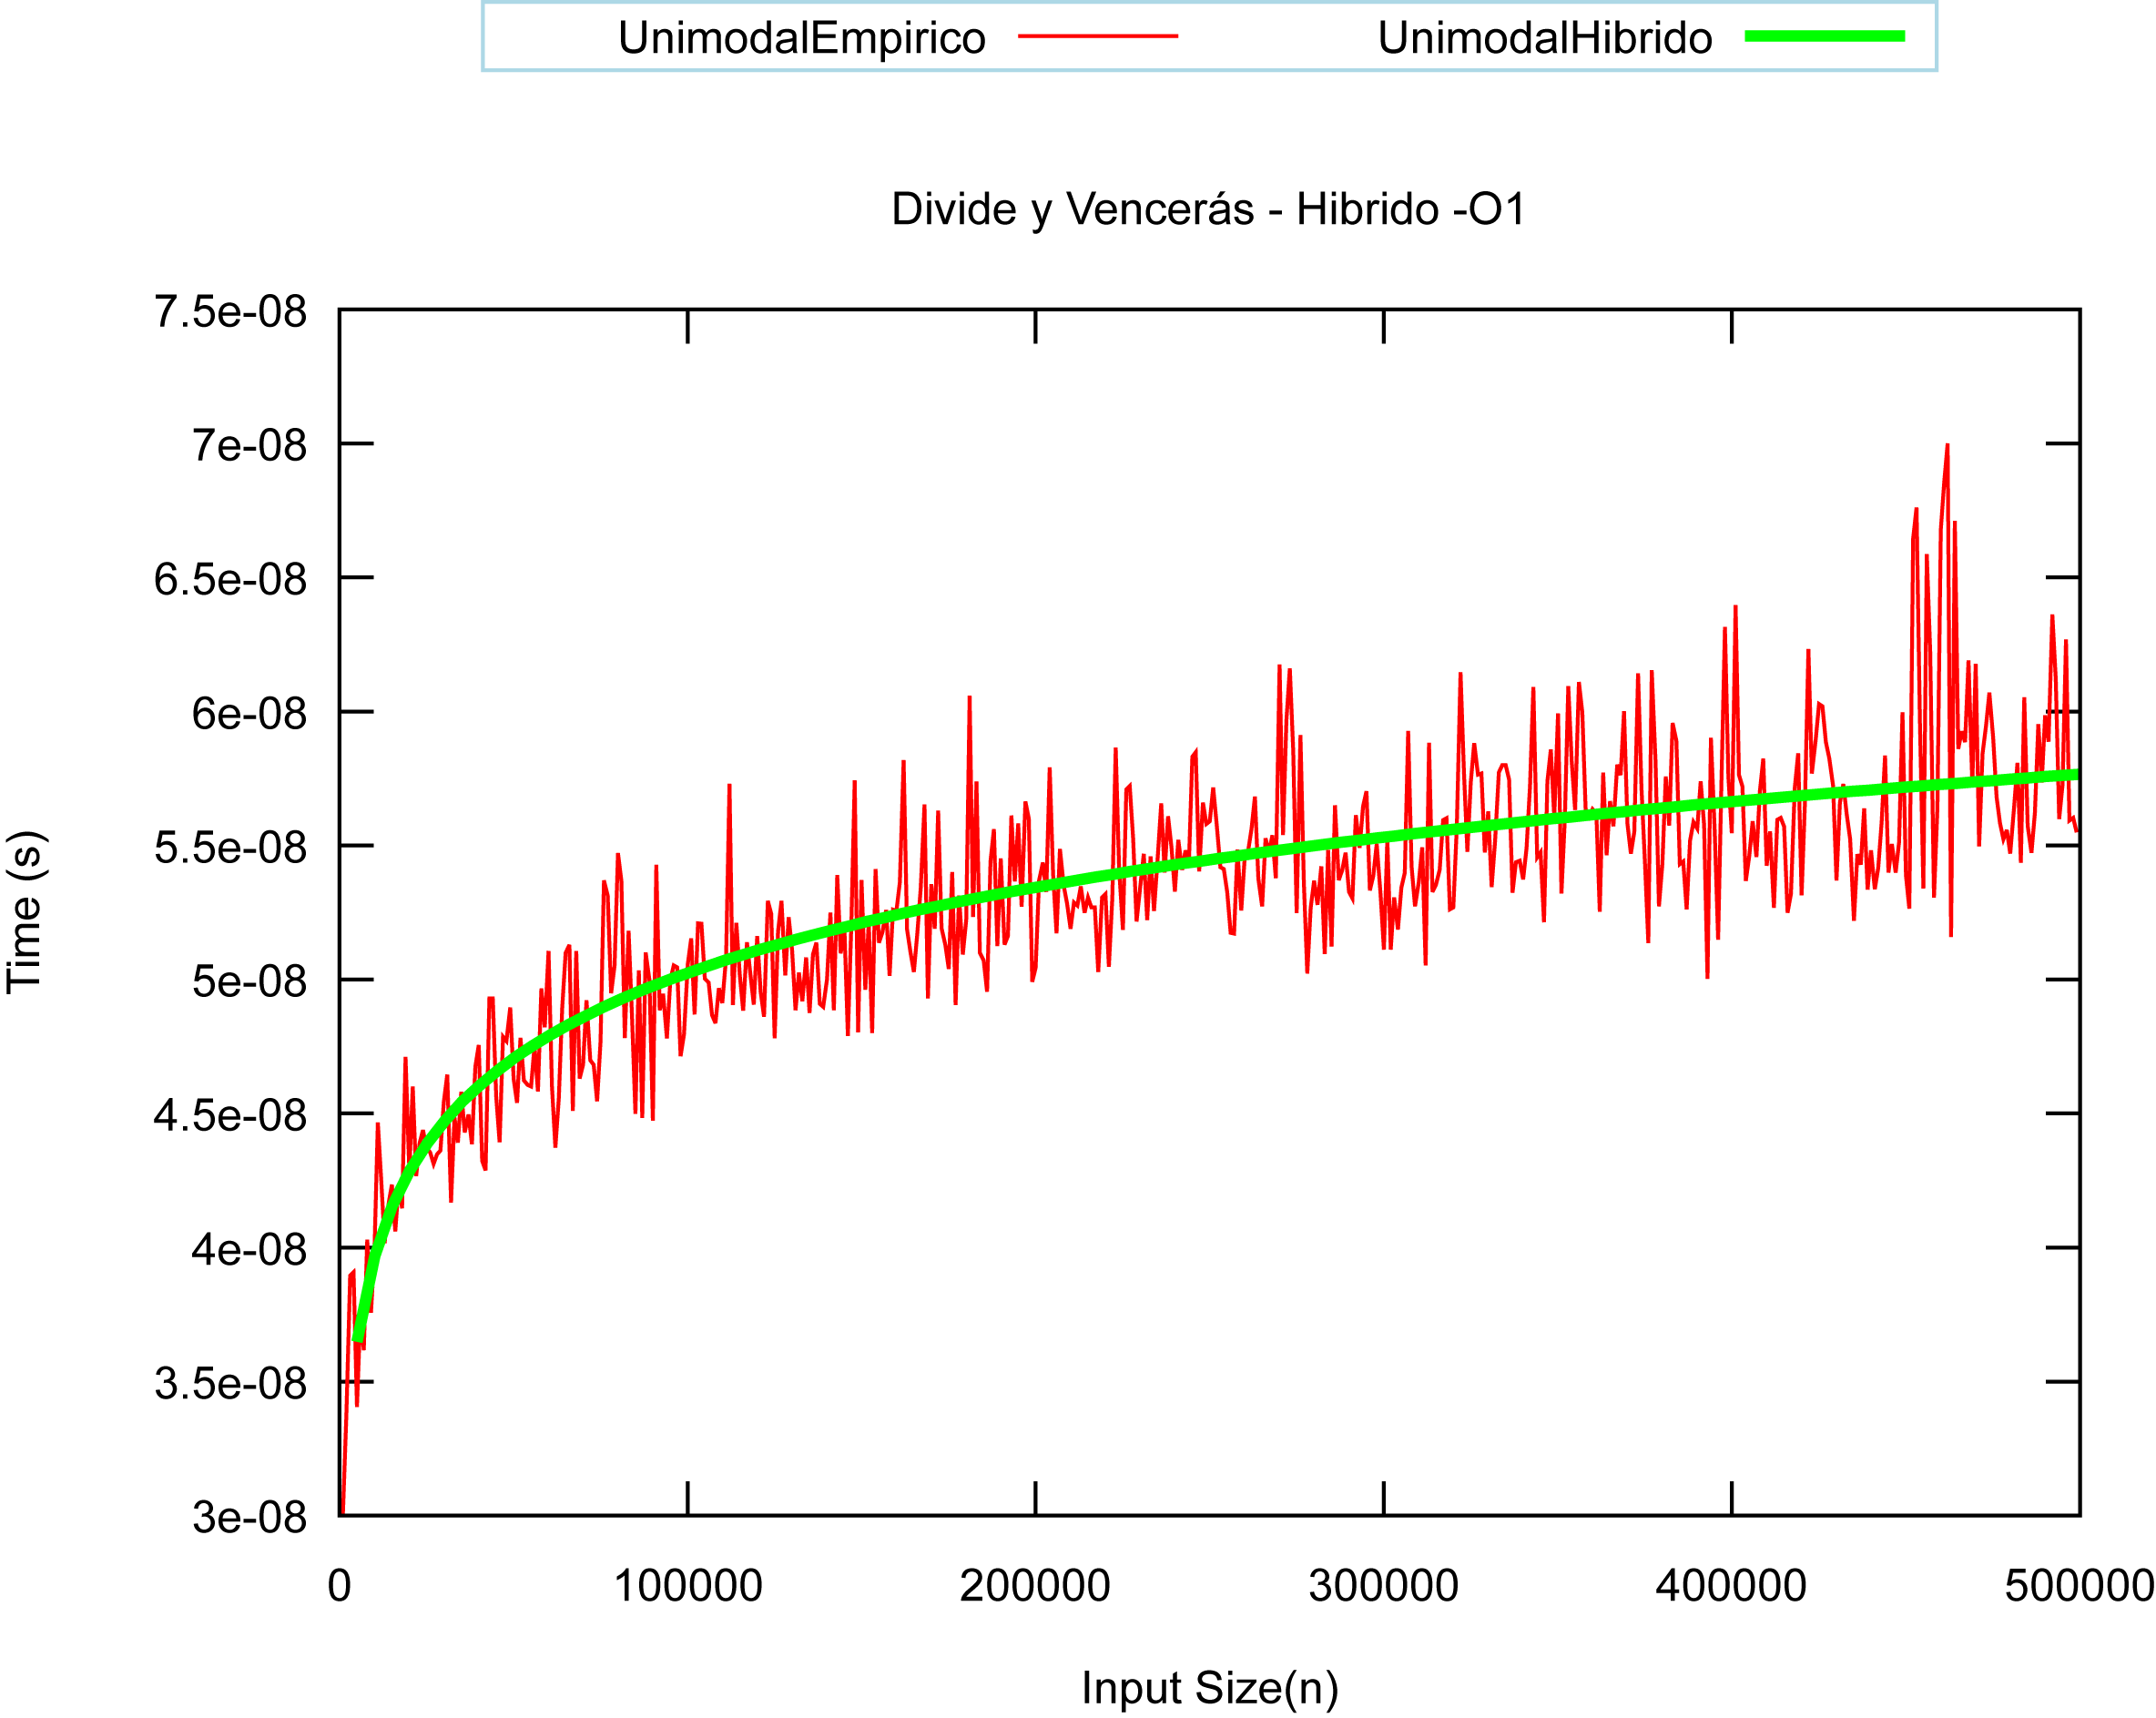
\includegraphics[width=8.6cm,height=7.1cm]{Images/dyv-hibridoO1}}
		\end{picture}
		\end{center}
		\end{figure}
		
\end{frame}	




\begin{frame}[plain]
	\frametitle{Constantes ocultas}
	
		\begin{defn}
			
			En este caso la función queda de la siguiente forma:
		
		\begin{equation}
			T(n) = 4.61006\cdot 10^{-09} \cdot log(n) - 2.83008\cdot 10^{-09}
		\end{equation}
	
		\vspace*{0.05in}
		
	\end{defn}
	
	

		
\end{frame}





\begin{frame}[plain]
	\frametitle{Optimización 2}
		\begin{figure}[htb]
		\begin{center}
		\begin{picture}(160,0)
		\put(-50,-110){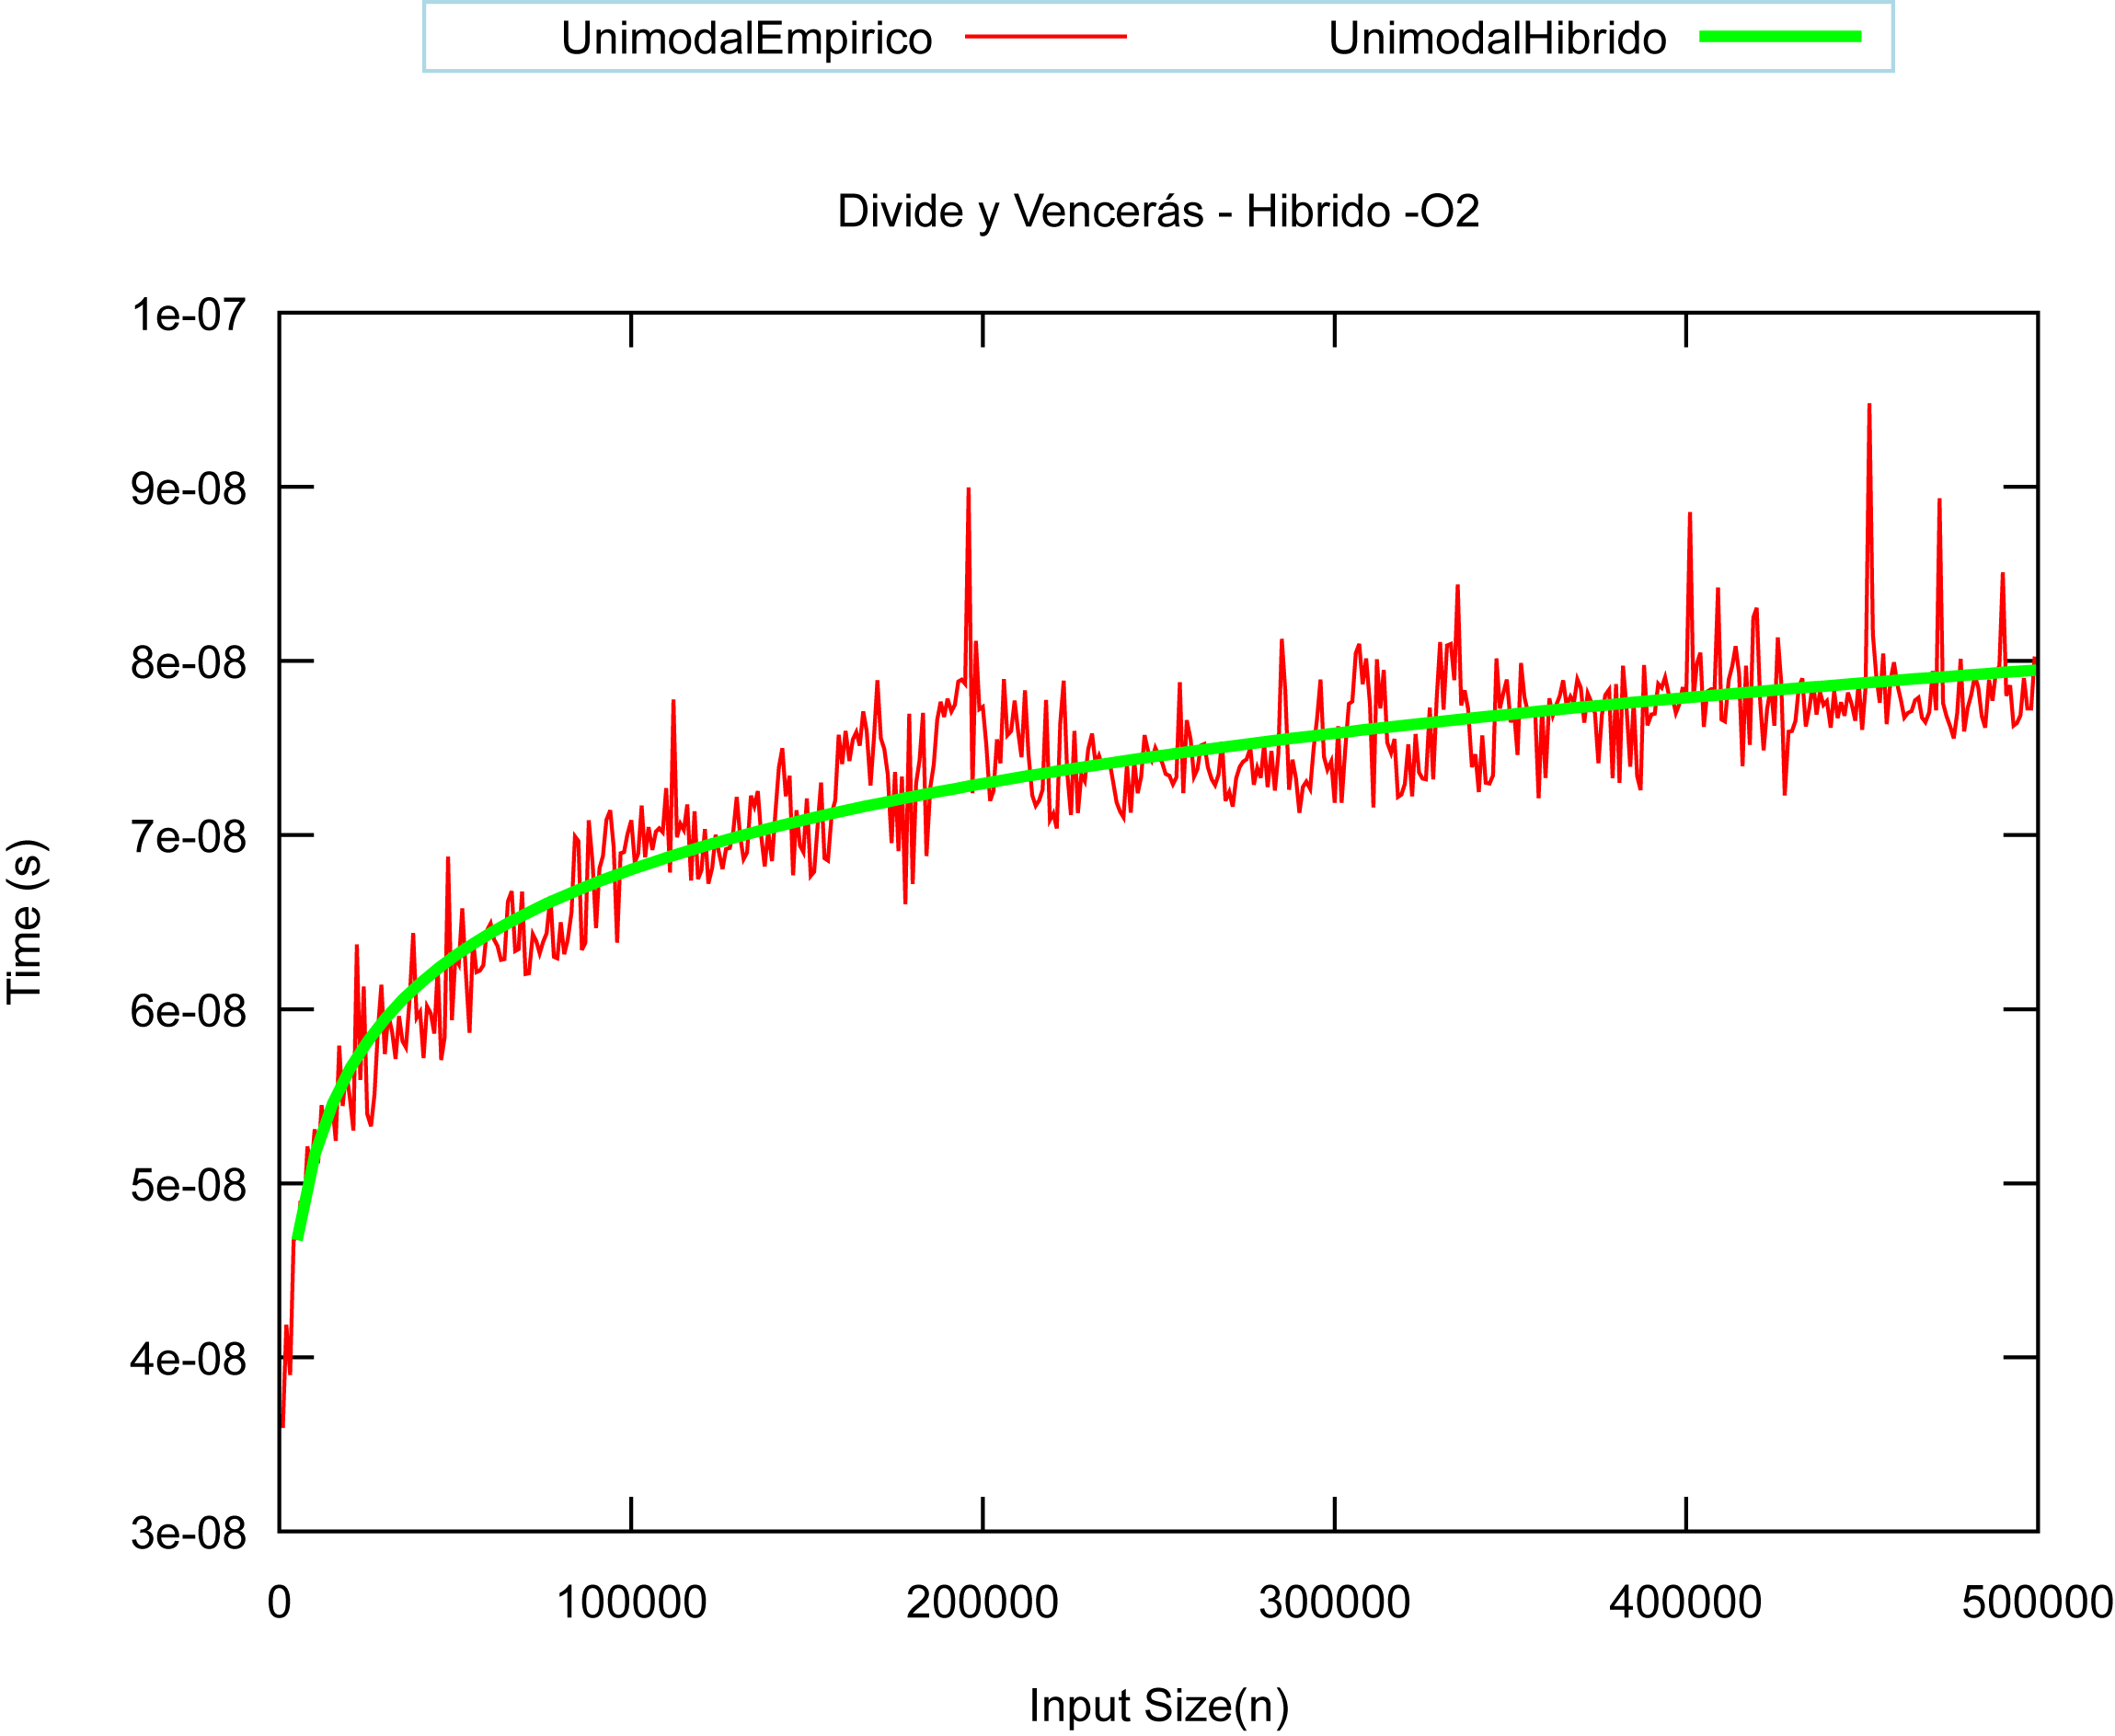
\includegraphics[width=8.6cm,height=7.1cm]{Images/dyv-hibridoO2}}
		\end{picture}
		\end{center}
		\end{figure}
		
\end{frame}	




\begin{frame}[plain]
	\frametitle{Constantes ocultas}
	
		\begin{defn}
			
			En este caso la función queda de la siguiente forma:
		
		\begin{equation}
			T(n) = 7.12567\cdot 10^{-09}  \cdot log(n) -1.4022\cdot 10^{-08} 
		\end{equation}
	
		\vspace*{0.05in}
		
	\end{defn}
	
	

		
\end{frame}







\begin{frame}[plain]
	\frametitle{Conclusión} 
	
	\begin{exampleblock}{Mejora}
			De nuevo, volvemos a ver que la mejoría se encuentra, como no podía ser de otra forma, en el valor de las constantes ocultas.
			También podemos observar que la mejoría es menos notoria si la comparamos con la mejora obtenida después de optimizar el algoritmo bruto hacia la optimización 1.
		\end{exampleblock}
\end{frame}		


		
		
		
	



